\section{Introduction and Recap of the Research Problem}
\label{sec:intro}

The previous workshop framed a study of how well a vision transformer reads the formal geometric relations contained in a textbook geometry diagram. Given a diagram and a named group of primitives (two segments, a point and a circle, or a segment and a circle), the task is to decide which relations hold between them: \rel{parallel}, \rel{perpendicular}, \rel{equal\_length}, \rel{on\_circle}, \rel{tangent} or \rel{collinear}. The defining choice is the reference against which correctness is judged. The datasets of the field record the relations an annotator chose to mark, usually because a symbol is printed in the figure \cite{lu2021intergps,zhang2022pgdp,zhang2023pgps}; this convention dates back to the first geometry solver \cite{seo2015geos}; this study instead takes the geometry of the drawing itself, measured from the coordinates of its points, as the ground truth, and compares it with the human annotation (Fig.~\ref{fig:recap}).

\begin{figure}[tbp]
  \centering
  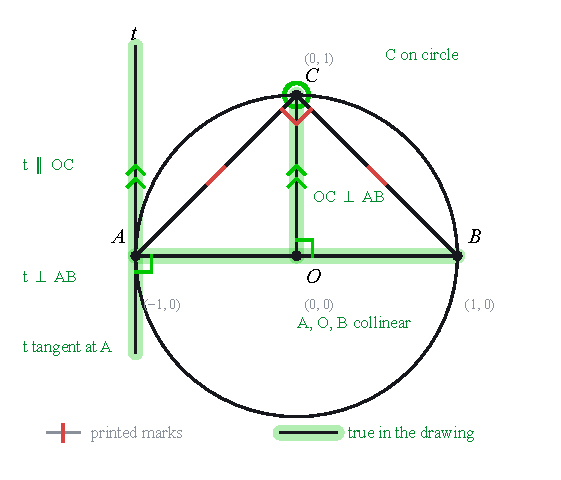
\includegraphics[width=0.6\textwidth]{fig_recap}
  \caption{One construction, two readings. Printed marks assert two relations (a right angle and two equal sides); the drawing satisfies six more that nobody marked (green). The verifier of Section~\ref{sec:preprocessing} labels all of them from the coordinates.}
  \label{fig:recap}
\end{figure}

The literature review identified four connected gaps. First, the ground truth in Geometry3K, PGDP5K and PGPS9K is the annotation, not the drawing, and a preliminary audit of the Geometry3K figures showed that most true relations are unmarked (\pctUnmarkedGParallel\% of the parallel pairs the drawings contain, \pctUnmarkedGPerpendicular\% of the perpendicular pairs, and all \nUnmarkedGTangent{} tangencies). Second, benchmark overlap hides generalisation: Geometry3K is split by problem rather than by figure, so \pctGeometryTestShareFigure\% of its test images share a figure with its training or validation split, and the three datasets reuse each other's images. Third, verifier-generated supervision, which lets AlphaGeometry train on unlimited correct synthetic data \cite{trinh2024alphageometry}, has never been applied to diagram perception. Fourth, perception is measured only indirectly, through problem answers \cite{zhang2024mathverse,gao2025gllava} or with annotated clauses in place of a parse \cite{zhang2023pgps}.

\paragraph{Problem statement.} \emph{Can a fine-tuned self-supervised vision transformer recognise the formal geometric relations that actually hold in a textbook diagram, when correctness is judged by a coordinate-based verifier rather than by human annotation; and does verifier-labelled synthetic data extend this ability to diagrams from an unseen source and to diagrams larger than any seen in training?}

\paragraph{Hypotheses.} \Hone: adding verifier-labelled synthetic diagrams to the real training data increases a fine-tuned vision transformer's macro-F1, measured against verifier labels, on (a) diagrams from an unseen source and (b) diagrams with more points than any training diagram, compared with training on real data alone at the same training budget. \Hzero: any difference in macro-F1 between the two training conditions is within the variation between random seeds. \Htwo: the same model scores substantially lower against human annotations than against verifier labels, and most of the difference comes from relations that hold in the drawing but are not marked.

This report turns that framing into a procedure. Section~\ref{sec:design} states the type of study and its variables; Sections~\ref{sec:dataset} and \ref{sec:preprocessing} describe the data and the pipeline that prepares it, including the verifier that produces the geometric labels; Sections~\ref{sec:model} and \ref{sec:training} give the model and the training plan with every setting; Section~\ref{sec:baselines} defines the comparisons; Section~\ref{sec:evaluation} the metrics and the decision rules for \Hone, \Hzero{} and \Htwo; and Section~\ref{sec:ethics} the ethical, bias and reproducibility provisions. Every quantity in the report is read from the project's configuration and data tables by a script, so that the text and the implementation cannot drift apart.
